\documentclass[a4paper,12pt]{article}  % Tipo de documento como artigo, com tamanho de fonte 12pt e formato A4
%Referência de Modelo para a FAI: https://www.fai-mg.br/biblio/images/publicacoes/modelo/ModeloArtigoCientifico.pdf %

\usepackage[brazil]{babel}  % Usa o idioma português (Brasil) para definir as convenções de idioma, como a separação de sílabas e tradução de termos.
\usepackage[utf8]{inputenc}  % Define a codificação de entrada como UTF-8 para permitir caracteres acentuados corretamente.
\usepackage[T1]{fontenc}  % Define a codificação de saída de fontes como T1, permitindo o uso correto de caracteres especiais.
\usepackage{times}     % Fonte Times New Roman
\usepackage{parskip}   % Remove a identação dos parágrafos
\usepackage{geometry}  % Permite personalizar as margens e o layout da página.
\usepackage{graphicx}  % Permite inserir gráficos, imagens e ajustar o tamanho deles.
\usepackage{titlesec}  % Fornece comandos para personalizar o formato dos títulos das seções.
\usepackage{fancyhdr}  % Permite personalizar os cabeçalhos e rodapés do documento.
\usepackage{setspace}  % Controla o espaçamento entre linhas no documento (aqui é usado para espaçamento de 1,5 linha).
\usepackage{csquotes}  % Fornece suporte para citações, garantindo que o estilo de aspas seja correto em diferentes idiomas.
\usepackage{ragged2e}  % Fornece comandos para justificar ou ajustar o alinhamento de texto.
\usepackage{lipsum}    % Para gerar texto Lorem Ipsum
\usepackage{enumitem} % Customizar alíneas
\usepackage[toc,page]{appendix} % Para gerenciar apêndices
\usepackage{pgfmath} % Para cálculos matemáticos nos apêndices
\usepackage{tabularx}
\usepackage{calc}

\setlength{\parindent}{0pt}  % Paragráfos sem identação, conforme modelo da FAI
\setstretch{1.5}  % This also sets 1.5 line spacing
\setlength{\parskip}{12pt}  % Espaçament ode 12pt entre paragrafos

% Define a numeração da página
\fancypagestyle{numbered}{
    \fancyhf{}
    \fancyhead[R]{{\fontsize{10pt}{12pt}\selectfont\thepage}}
    \renewcommand{\headrulewidth}{0pt}
}

% Quanto à separação entre títulos, subtítulos e texto, observa-se o seguinte:
\let\oldsection\section
\renewcommand{\section}[1]{%
    \clearpage % os títulos de capítulos estão sempre no início de uma nova página;
    \thispagestyle{empty} % No page number on this page
    \oldsection{#1}
}
% seções primárias: os títulos dessas seções devem ser em caixa alta, fonte 12 e em negrito;
\titleformat{\section}{\normalfont\fontsize{12}{12}\selectfont\bfseries}{\thesection}{0.3em}{\MakeUppercase}

\let\oldsubsection\subsection
\renewcommand{\subsection}[1]{%
    \par\vspace{2\parskip}
    \oldsubsection{#1}
    \par\vspace{0.5\parskip} % separação entre o texto e os subtítulos: pula-se uma linha em branco.
}
% seções secundárias: os títulos dessas seções devem ser iguais aos das primárias, porém sem negrito;
\titleformat{\subsection}{\normalfont\fontsize{12}{12}\selectfont}{\thesubsection}{0.3em}{\MakeUppercase}

% Define spacing for subsubsection
\let\oldsubsubsection\subsubsection
\renewcommand{\subsubsection}[1]{%
    \par\vspace{2\parskip}
    \oldsubsubsection{#1}
    \par\vspace{0.5\parskip}% Add paragraph break after
}
% seções terciárias: os títulos dessas seções devem ser em negrito, somente com a primeira letra maiúscula;
\titleformat{\subsubsection}{\normalfont\fontsize{12}{14.4}\bfseries}{\thesubsubsection}{0.3em}{}

\geometry{
    left=3cm,
    right=2cm,
    top=3cm,
    bottom=2cm,
    headsep=35pt,
    footskip=0pt
    % , showframe
} % Define as margens da página (esquerda = 3cm, direita = 2cm, topo = 3cm, fundo = 2cm)

% Configuração das alíneas
\newlist{alinea}{enumerate}{1}
\setlist[alinea,1]{
    label=\alph*), % c) as alíneas devem ser indicadas alfabeticamente, em letra minúscula, seguida de parêntese fechado. Utilizam-se letras dobradas, quando esgotadas as letras do alfabeto;
    leftmargin=1cm,        % Total indentation from current margin
    itemindent=0pt,        % No additional item indentation
    labelsep=0pt,          % No space between label and text
    labelwidth=13pt,       % d) as letras indicativas das alíneas devem apresentar recuo de 0,5 cm em relação à margem esquerda;
    itemsep=0pt,
    parsep=0pt,
    topsep=0pt,
    partopsep=0pt,
    align=left,
    before={\setlength{\parskip}{0pt}},  % h) Entre as alíneas, inclusive a primeira delas, os parágrafos são formatados com zero ponto ante e zero depois
    after={\setlength{\parskip}{12pt}}   % i) O próximo parágrafo, após a última alínea, volta a ter formatação normal com 12 pontos antes e 12 depois.
}

\newcommand{\listaalinhada}[2]{%
  \noindent%
  \begin{tabularx}{\textwidth}{lX}
  {#1}: & \parbox[t]{\linewidth}{\raggedright #2}
  \end{tabularx}%
  \\
}

\usepackage[style=authoryear, sorting=nyt, backend=bibtex]{biblatex}  % Carrega o pacote BibLaTeX para bibliografia e define o estilo de ordenação como "nyt" (nome, ano, título).
\renewcommand*{\bibfont}{\raggedright\singlespacing}  % Alinha a bibliografia à esquerda com espaçamento simples.
\setlength{\bibhang}{0pt}

% Configurações para formato ABNT
\DeclareFieldFormat{title}{\textbf{#1}}
\DeclareFieldFormat[article]{title}{\textbf{#1}}
\DeclareNameAlias{sortname}{family-given}
\DeclareFieldFormat{nameyeardelim}{\addcomma\space}

% Formato do nome: SOBRENOME, Nome
\DeclareNameFormat{family-given}{%
  \ifgiveninits
    {\usebibmacro{name:family-given}
      {\namepartfamily}
      {\namepartgiveni}
      {\namepartprefix}
      {\namepartsuffix}}
    {\usebibmacro{name:family-given}
      {\namepartfamily}
      {\namepartgiven}
      {\namepartprefix}
      {\namepartsuffix}}%
  \usebibmacro{name:andothers}}

\renewbibmacro*{name:family-given}[4]{%
  \ifuseprefix
    {\usebibmacro{name:delim}{#3#1}%
     \usebibmacro{name:hook}{#3#1}%
     \ifblank{#3}{}{%
       \ifcapital
         {\mkbibnameprefix{\MakeCapital{#3}}\isdot}
         {\mkbibnameprefix{#3}\isdot}%
       \ifpunctmark{'}{}{\bibnamedelimc}}%
     \mkbibnamefamily{\MakeUppercase{#1}}\isdot
     \ifblank{#2}{}{\revsdnamepunct\bibnamedelimd\mkbibnamegiven{#2}\isdot}%
     \ifblank{#4}{}{\bibnamedelimd\mkbibnamesuffix{#4}\isdot}}
    {\usebibmacro{name:delim}{#1}%
     \usebibmacro{name:hook}{#1}%
     \mkbibnamefamily{\MakeUppercase{#1}}\isdot
     \ifblank{#2}{}{\revsdnamepunct\bibnamedelimd\mkbibnamegiven{#2}\isdot}%
     \ifblank{#4}{}{\bibnamedelimd\mkbibnamesuffix{#4}\isdot}}}

% Remove parênteses do ano e coloca no final
\renewbibmacro*{date+extradate}{%
  \iffieldundef{labelyear}
    {}
    {\printtext{\printfield{labelyear}%
     \printfield{extradate}}}}

% Redefine o driver para livros (books)
\DeclareBibliographyDriver{book}{%
  \usebibmacro{bibindex}%
  \usebibmacro{begentry}%
  \usebibmacro{author/editor+others/translator+others}%
  \setunit{\labelnamepunct}\newblock
  \usebibmacro{maintitle+title}%
  \newunit
  \printlist{language}%
  \newunit\newblock
  \usebibmacro{byauthor}%
  \newunit\newblock
  \usebibmacro{byeditor+others}%
  \newunit\newblock
  \printfield{edition}%
  \newunit
  \iflistundef{location}
    {}
    {\printlist{location}}%
  \iflistundef{publisher}
    {}
    {\setunit*{\addcolon\space}%
     \printlist{publisher}}%
  \setunit*{\addcomma\space}%
  \usebibmacro{date+extradate}%
  \newunit\newblock
  \iftoggle{bbx:isbn}
    {\printfield{isbn}}
    {}%
  \newunit\newblock
  \usebibmacro{doi+eprint+url}%
  \newunit\newblock
  \usebibmacro{addendum+pubstate}%
  \setunit{\bibpagerefpunct}\newblock
  \usebibmacro{pageref}%
  \newunit\newblock
  \iftoggle{bbx:related}
    {\usebibmacro{related:init}%
     \usebibmacro{related}}
    {}%
  \usebibmacro{finentry}}

% Redefine o título da seção de referências para maiúsculas e centralizado
\defbibheading{bibliography}{%
  \begin{center}
    \textbf{\MakeUppercase{Referências}}
  \end{center}
}

% Customização do Sumário ----------------------------------------------------------
\usepackage{tocloft}
\usepackage{xstring}
\usepackage{textcase}

\setcounter{tocdepth}{2} % Incluir apenas secao primaria e secundaria

\renewcommand{\contentsname}{SUMÁRIO}
\renewcommand{\cftsecfont}{\bfseries}
\renewcommand{\cftsecpagefont}{\bfseries}
\renewcommand{\cftsecleader}{\cftdotfill{\cftdotsep}}
\setlength{\cftbeforetoctitleskip}{0pt}
\setlength{\cftaftertoctitleskip}{0.4cm}
\renewcommand{\cfttoctitlefont}{\hfil\bfseries}


\renewcommand{\cfttoctitlefont}{\hfil\rmfamily\bfseries\MakeUppercase} % Título maiúsculo
\renewcommand{\cftdotsep}{0.1} % Adiciona mais pontos. Menor numero = Mais pontos
\setlength{\cftbeforesecskip}{0em} % Espaço entre as linhas de seção
\setlength{\cftbeforesubsecskip}{0em} % Espaço entre as linhas de subseção
\setlength{\cftbeforesubsubsecskip}{0em} % Espaço entre as linhas de subsubseção
\setlength{\cftsecindent}{0em} % Remove identação das seções
\setlength{\cftsubsecindent}{0em}   % Remove identação das subseções
\setlength{\cftsubsubsecindent}{0em} % Remove identação das subsubseções

\setlength{\cftsecnumwidth}{1.2em} % Espaço entre número da seção e texto
\setlength{\cftsubsecnumwidth}{1.5em} % Espaço entre número da subseção e texto
\setlength{\cftsubsubsecnumwidth}{2.3em} % Espaço entre número da subsubseção e texto

% Seção, subseção e subsubseção em maiúsculo no Sumário
\makeatletter
\let\oldcontentsline\contentsline
\renewcommand{\contentsline}[4]{%
  \expandafter\ifx\csname l@#1\endcsname\l@section
    \oldcontentsline{#1}{\MakeUppercase{#2}}{#3}{#4}%
  \else
    \expandafter\ifx\csname l@#1\endcsname\l@subsection
      \oldcontentsline{#1}{\MakeUppercase{#2}}{#3}{#4}%
    \else
      \expandafter\ifx\csname l@#1\endcsname\l@subsubsection
        \oldcontentsline{#1}{\MakeUppercase{#2}}{#3}{#4}%
      \else
        \oldcontentsline{#1}{#2}{#3}{#4}%
      \fi
    \fi
  \fi
}
\makeatother
% ------------------------------------------------------------------------------------

% Funções customizadas para criar e imprimir autores ---------------------------------
\usepackage{pgffor}

\newcounter{authorcount} % Counter para autores

% Comando para adicionar novos autores
\newcommand{\AdicionarAutor}[2]{% #1 = nome, #2 = email
    \stepcounter{authorcount}
    \expandafter\def\csname author\theauthorcount\endcsname{#1}
    \expandafter\def\csname email\theauthorcount\endcsname{#2}
}

% Comando para imprimir os autores
\newcommand{\imprimirautores}{%
    \foreach \i in {1,...,\theauthorcount} {%
        \textbf{\fontsize{12}{14}\selectfont\MakeUppercase{\csname author\i\endcsname}} \\
    }%
}

%  ------------------------------------------------------------------------
\newcounter{avaliadorcount}

\newcommand{\AdicionarBancaExaminadora}[2]{%
    \stepcounter{avaliadorcount}
    \expandafter\def\csname tipo\theavaliadorcount\endcsname{#1}
    \expandafter\def\csname nome\theavaliadorcount\endcsname{#2}
}

\newcommand{\imprimirbancaexaminadora}{%
    \foreach \i in {1,...,\theavaliadorcount} {%
        \underline{\hspace*{8cm}} \\
        \textbf{\fontsize{12}{14}\selectfont{\csname tipo\i\endcsname}} \textbf{\fontsize{12}{14}\selectfont{\csname nome\i\endcsname}} \\[2em]
    }%
}

% ------------------------------------------------------------------------------------

% Funções para Citação Direta ---------------------------------
\newenvironment{citacaodireta}
{\par\addvspace{\baselineskip}% Add exactly one line space before
 \begingroup
 \list{}{\leftmargin=4cm
         \rightmargin=0pt
         \parsep=0pt
         \itemsep=0pt
         \topsep=0pt}
 \item\relax
 \singlespacing
 \fontsize{10}{12}\selectfont
 \justifying}
{\endlist
 \endgroup
 \par\addvspace{\baselineskip}}% Add exactly one line space after

% Usar:
% \begin{citacaodireta}
% ...
% \end{citacaodireta}
% ------------------------------------------------------------------------------------

% Customização das Listas de Ilustrações ---------------------------------
\usepackage[labelfont=bf]{caption}
\usepackage{newfloat} % Para criar novos tipos de float

% Definir novos tipos de float
\DeclareFloatingEnvironment[
    fileext=fig,
    listname={Lista de Figuras},
    name=Figura,
    placement=htbp,
]{figura}

\DeclareFloatingEnvironment[
    fileext=fot,
    listname={Lista de Fotografias},
    name=Fotografia,
    placement=htbp,
]{fotografia}

\DeclareFloatingEnvironment[
    fileext=grf,
    listname={Lista de Gráficos},
    name=Gráfico,
    placement=htbp,
]{grafico}

\DeclareFloatingEnvironment[
    fileext=qua,
    listname={Lista de Quadros},
    name=Quadro,
    placement=htbp,
]{quadro}

% Contadores para cada tipo
\newcounter{totalfiguras}
\newcounter{totalfotografias}
\newcounter{totalgraficos}
\newcounter{totalquadros}

% Comandos para incrementar contadores
\newcommand{\addfigura}{\stepcounter{totalfiguras}}
\newcommand{\addfotografia}{\stepcounter{totalfotografias}}
\newcommand{\addgrafico}{\stepcounter{totalgraficos}}
\newcommand{\addquadro}{\stepcounter{totalquadros}}

% Sistema de duas passadas para listas condicionais
\makeatletter
% Escrever contadores no arquivo auxiliar ao final do documento
\AtEndDocument{%
    \immediate\write\@auxout{\string\gdef\string\@totalfiguras{\arabic{totalfiguras}}}%
    \immediate\write\@auxout{\string\gdef\string\@totalfotografias{\arabic{totalfotografias}}}%
    \immediate\write\@auxout{\string\gdef\string\@totalgraficos{\arabic{totalgraficos}}}%
    \immediate\write\@auxout{\string\gdef\string\@totalquadros{\arabic{totalquadros}}}%
}

% Definir valores padrão se não existirem (primeira compilação)
\@ifundefined{@totalfiguras}{\gdef\@totalfiguras{0}}{}
\@ifundefined{@totalfotografias}{\gdef\@totalfotografias{0}}{}
\@ifundefined{@totalgraficos}{\gdef\@totalgraficos{0}}{}
\@ifundefined{@totalquadros}{\gdef\@totalquadros{0}}{}

% Comandos condicionais usando os valores da compilação anterior
\newcommand{\ifhasfiguras}[2]{\ifnum\@totalfiguras>0 #1\else #2\fi}
\newcommand{\ifhasfotografias}[2]{\ifnum\@totalfotografias>0 #1\else #2\fi}
\newcommand{\ifhasgraficos}[2]{\ifnum\@totalgraficos>0 #1\else #2\fi}
\newcommand{\ifhasquadros}[2]{\ifnum\@totalquadros>0 #1\else #2\fi}
\makeatother
% ------------------------------------------------------------------------------------

% Customização da Lista de Figuras ---------------------------------
\usepackage[labelfont=bf]{caption}
\usepackage[figure]{totalcount} % Add this package
\makeatletter
\renewcommand{\@cftmakeloftitle}{} % Completely remove title generation
\makeatother

% Configure the figure entries with uppercase and dash
\renewcommand{\cftfigpresnum}{FIGURA }
\renewcommand{\cftfigaftersnum}{ -- }
\setlength{\cftfignumwidth}{2.5cm} % Adjust width for new format
\setlength{\cftfigindent}{0pt} % No indentation

% Define formatting for other illustration types
% The newfloat package creates \l@<environment> commands that we can customize
\makeatletter
% Custom formatting for quadro entries
\renewcommand*{\l@quadro}[2]{%
  \ifnum \c@tocdepth >\z@
    \addpenalty\@secpenalty
    \setlength\@tempdima{0.5cm}%
    \begingroup
      \parindent \z@ \rightskip \@pnumwidth
      \parfillskip -\@pnumwidth
      \leavevmode
      \advance\leftskip\@tempdima
      \hskip -\leftskip
      % --- The robust fix is here ---
      \def\numberline##1##2{%
        QUADRO ##1{} -- ##2%
      }%
      #1%
      \nobreak
      % --- End of fix ---
      \renewcommand{\@dotsep}{0.3}%
      \leaders\hbox{$\m@th\mkern \@dotsep mu\hbox{.}\mkern \@dotsep mu$}\hfill
      \nobreak\hb@xt@\@pnumwidth{\hss #2}\par
    \endgroup
  \fi}

% Custom formatting for fotografia entries  
% Custom formatting for fotografia entries
\renewcommand*{\l@fotografia}[2]{%
  \ifnum \c@tocdepth >\z@
    \addpenalty\@secpenalty
    \setlength\@tempdima{3cm}%
    \begingroup
      \parindent \z@ \rightskip \@pnumwidth
      \parfillskip -\@pnumwidth
      \leavevmode
      \advance\leftskip\@tempdima
      \hskip -\leftskip
      % --- The robust fix is here ---
      \def\numberline##1##2{%
        FOTOGRAFIA ##1 -- ##2%
      }%
      #1%
      \nobreak
      % --- End of fix ---
      \renewcommand{\@dotsep}{0.5}%
      \leaders\hbox{$\m@th\mkern \@dotsep mu\hbox{.}\mkern \@dotsep mu$}\hfill
      \nobreak\hb@xt@\@pnumwidth{\hss #2}\par
    \endgroup
  \fi}

% Custom formatting for grafico entries
\renewcommand*{\l@grafico}[2]{%
  \ifnum \c@tocdepth >\z@
    \addpenalty\@secpenalty
    \setlength\@tempdima{2.5cm}%
    \begingroup
      \parindent \z@ \rightskip \@pnumwidth
      \parfillskip -\@pnumwidth
      \leavevmode
      \advance\leftskip\@tempdima
      \hskip -\leftskip
      % --- The robust fix is here ---
      \def\numberline##1##2{%
        GRÁFICO ##1 -- ##2%
      }%
      #1%
      \nobreak
      % --- End of fix ---
      \renewcommand{\@dotsep}{0.5}%
      \leaders\hbox{$\m@th\mkern \@dotsep mu\hbox{.}\mkern \@dotsep mu$}\hfill
      \nobreak\hb@xt@\@pnumwidth{\hss #2}\par
    \endgroup
  \fi}
\makeatother

% Note: List formatting for other illustration types (fotografia, grafico, quadro)
% is handled by the newfloat package automatically. The caption formatting
% below will ensure consistent appearance in both captions and lists.
% ------------------------------------------------------------------------------------

\usepackage{caption}

\newcommand{\fonte}[1]{%
  \vspace{0em}%
  \begin{minipage}{\textwidth}%
    \raggedright%
    \footnotesize%
    FONTE: #1%
  \end{minipage}%
}

% Create \legenda as alias for \caption with full functionality
\NewCommandCopy{\legenda}{\caption}

% Create \equacao as alias for \equacao with full functionality
\newenvironment{equacao}{\begin{equation}}{\end{equation}}

% Custom caption formatting for all illustration types
% Using footnote size, capital letters, and dash separator
\captionsetup[quadro]{
    justification=raggedright,
    singlelinecheck=false,
    font={footnotesize},
    labelfont={footnotesize},
    labelformat=simple,
    labelsep=none,
    format=plain
}

\captionsetup[figura]{
    justification=raggedright,
    singlelinecheck=false,
    font={footnotesize},
    labelfont={footnotesize},
    labelformat=simple,
    labelsep=none,
    format=plain
}

\captionsetup[grafico]{
    justification=raggedright,
    singlelinecheck=false,
    font={footnotesize},
    labelfont={footnotesize},
    labelformat=simple,
    labelsep=none,
    format=plain
}

\captionsetup[fotografia]{
    justification=raggedright,
    singlelinecheck=false,
    font={footnotesize},
    labelfont={footnotesize},
    labelformat=simple,
    labelsep=none,
    format=plain
}

% Custom label formatting to use uppercase names with dashes
\DeclareCaptionLabelFormat{customdash}{\MakeUppercase{#1} #2 - }

% Apply custom label format to all illustration types
\captionsetup[quadro]{labelformat=customdash}
\captionsetup[figura]{labelformat=customdash}
\captionsetup[grafico]{labelformat=customdash}
\captionsetup[fotografia]{labelformat=customdash}

% Definição de funções em português de acordo com a nomeclatura da FAI
\let\secaoprimaria\section
\let\secaosecundaria\subsection
\let\secaoterciaria\subsubsection


\addbibresource{referencias/referencias.bib}  % Adiciona o arquivo de bibliografia (referencias/referencias.bib) como fonte para as referências bibliográficas. % Definições de formato e estilo do documento seguindo diretrizes da FAI
% Define o tipo de Documento. Usado para condicionar elementos textuais
\def\@monografia{Monografia}
\def\@projeto{Projeto de Pesquisa}
\def\@relatorio{Relatório de Estágio}
\def\@trabalhos{Trabalhos acadêmicos}

% Definições por grupos de elementos textuais
\newenvironment{ElementosPreTextuais}{
    \pagestyle{numbered}
}{}

\newenvironment{ElementosTextuais}{
    \clearpage
    \setcounter{savepage}{\value{page}} % Salva o número da página atual
    \pagenumbering{arabic}
    \setcounter{page}{\value{savepage}} % Restaura o número da página
    \pagestyle{numbered}
}{
    \newpage
}

\newenvironment{ElementosPosTextuais}{
    \clearpage
    \pagestyle{numbered}
}{}

% Definições por tipos de conteúdo
\newenvironment{CapaOuFalsaFolhaDeRosto}{
    \pagenumbering{roman}
    \pagestyle{numbered}
    \setcounter{page}{1}
    \thispagestyle{empty} % Remove numeração da primeira página
    \begin{center}
}{
    \textbf{\instituicao}

    \textbf{\curso}

    \vfill

    \imprimirautores
    
    \vfill

    \textbf{\fontsize{12}{14}\selectfont\MakeUppercase{\titulo: \subtitulo}}
    
    \vfill

    \vspace{\theauthorcount\baselineskip} % Mesmo espaço da lista de autores para que o título fique centralizado
    
    \vfill

    \textbf{\local}\\
    \textbf{\ano}
    \end{center}
    \newpage
}

\newenvironment{FolhaDeRosto}{
    \begin{center}
}{
    \textbf{\instituicao}

    \textbf{\curso}
    
    \vspace{2\baselineskip}

    \vfill

    \imprimirautores

    \vspace{2\baselineskip}

    
    \vfill
    
    \textbf{\fontsize{12}{14}\selectfont\MakeUppercase{\titulo: \subtitulo}}
    
    \vfill

    {\singlespacing\justifying\hspace{7cm}\parbox{\dimexpr\textwidth-7cm}{
    \natureza
    }}

    \vfill
    \textbf{\local}\\
    \textbf{\ano}
    \end{center}
    \newpage
}

\newenvironment{FolhaDeAprovacao}{
    \begin{center}
    \fontsize{12}{14}\selectfont
    \bfseries
}{
    \instituicao

    \curso

    \end{center}

    \vfill

    \textbf{AUTORES:} \imprimirautores
    \textbf{TÍTULO:} \textbf{\fontsize{12}{14}\selectfont\MakeUppercase{\titulo}}

    \vfill
    
    \textbf{BANCA EXAMINADORA}

    \vspace{2\baselineskip}

    \imprimirbancaexaminadora

    \textbf\local \quad \textbf{\fontsize{12}{14}\selectfont\MakeUppercase{\_\_/\_\_/\_\_.}}

    \newpage
}

\newenvironment{Dedicatoria}{
    \vspace*{\fill}
    \begin{flushright}
    \begin{minipage}{0.5\textwidth}
    \raggedleft
    \singlespacing
    \justifying
}{
    \end{minipage}
    \end{flushright}
    \vspace{1cm}
    \newpage
}

\newenvironment{Agradecimentos}{
    \begin{center}
    \textbf{AGRADECIMENTOS}
    \end{center}
    \noindent
}{
    \newpage
}

\newenvironment{Epigrafe}{
    \vspace*{\fill}
    \begin{flushright}
    \begin{minipage}{0.5\textwidth}
    \raggedleft
    \singlespacing
    \justifying
}{
    \end{minipage}
    \end{flushright}
    \vspace{1cm}
    \newpage
}

\newenvironment{Resumo}{
    \begin{center}
    \textbf{RESUMO}
    \end{center}
    
    \justifying
    \begin{singlespace}
    \resumo
    \end{singlespace}
    
    \textbf{Palavras-chave:} \palavraschave
    
    \vspace{1cm}
    \begin{center}
    \textbf{ABSTRACT}
    \end{center}
    
    \justifying
    \begin{singlespace}
    \resumoingles
    \end{singlespace}
    
    \textbf{Keywords:} \palavraschaveingles
}{
    \newpage
}


% Comandos para listas condicionais de ilustrações
% Usando sistema de duas passadas com arquivo auxiliar

% Comandos auxiliares para verificar quantidades
\makeatletter
\newcommand{\ifmorethanninefiguras}[2]{\ifnum\@totalfiguras>9\relax #1\else #2\fi}
\newcommand{\ifmorethanninetotos}[2]{\ifnum\@totalfotografias>9\relax #1\else #2\fi}
\newcommand{\ifmorethanninegraficos}[2]{\ifnum\@totalgraficos>9\relax #1\else #2\fi}
\newcommand{\ifmorethanninequadros}[2]{\ifnum\@totalquadros>9\relax #1\else #2\fi}

\newcommand{\iflessthantenfiguras}[2]{\ifnum\@totalfiguras<10\relax #1\else #2\fi}
\newcommand{\iflessthantenfotos}[2]{\ifnum\@totalfotografias<10\relax #1\else #2\fi}
\newcommand{\iflessthantengraficos}[2]{\ifnum\@totalgraficos<10\relax #1\else #2\fi}
\newcommand{\iflessthantenquadros}[2]{\ifnum\@totalquadros<10\relax #1\else #2\fi}

\newcommand{\ifhasanyillustration}[2]{%
  \newif\ifanyillustration%
  \anyillustrationfalse%
  \ifnum\@totalfiguras>0\relax \ifnum\@totalfiguras<10\relax \anyillustrationtrue\fi\fi%
  \ifnum\@totalfotografias>0\relax \ifnum\@totalfotografias<10\relax \anyillustrationtrue\fi\fi%
  \ifnum\@totalgraficos>0\relax \ifnum\@totalgraficos<10\relax \anyillustrationtrue\fi\fi%
  \ifnum\@totalquadros>0\relax \ifnum\@totalquadros<10\relax \anyillustrationtrue\fi\fi%
  \ifanyillustration#1\else#2\fi%
}

\makeatother

% Lista unificada de ilustrações (quando há menos de 2 de algum tipo)
\newcommand{\ListaDeIlustracoes}{%
    % Verifica se alguma categorias têm menos de 9 itens
    \ifhasanyillustration{%
        \clearpage
        \begin{center}
        \textbf{LISTA DE ILUSTRAÇÕES}
        \vspace{0.3cm}
        \end{center}
        % Inclui figuras se existirem
        \iflessthantenfiguras{\listoffigura}{}%
        % Inclui fotografias se existirem
        \iflessthantenfotos{\listoffotografia}{}%
        % Inclui gráficos se existirem
        \iflessthantengraficos{\listofgrafico}{}%
        % Inclui quadros se existirem
        \iflessthantenquadros{\listofquadro}{}%
        \clearpage
    }{}%
}

\newcommand{\ListaDeFiguras}{%
    % Só mostra lista individual se há 10 ou mais figuras
    \ifmorethanninefiguras{%
        \clearpage
        \begin{center}
        \textbf{LISTA DE FIGURAS}
        \vspace{0.3cm}
        \end{center}
        \listoffigura
        \clearpage
    }{}%
}

\newcommand{\ListaDeFotografias}{%
    % Só mostra lista individual se há 10 ou mais fotografias
    \ifmorethanninetotos{%
        \clearpage
        \begin{center}
        \textbf{LISTA DE FOTOGRAFIAS}
        \vspace{0.3cm}
        \end{center}
        \listoffotografia
        \clearpage
    }{}%
}

\newcommand{\ListaDeGraficos}{%
    % Só mostra lista individual se há 10 ou mais gráficos
    \ifmorethanninegraficos{%
        \clearpage
        \begin{center}
        \textbf{LISTA DE GRÁFICOS}
        \vspace{0.3cm}
        \end{center}
        \listofgrafico
        \clearpage
    }{}%
}

\newcommand{\ListaDeQuadros}{%
    % Só mostra lista individual se há 10 ou mais quadros
    \ifmorethanninequadros{%
        \clearpage
        \begin{center}
        \textbf{LISTA DE QUADROS}
        \vspace{0.3cm}
        \end{center}
        \listofquadro
        \clearpage
    }{}%
}

\newenvironment{ListaDeTabelas}{
    
}{}

% ============================================================================
% SISTEMA DE SIGLAS E ABREVIATURAS AUTOMÁTICO
% ============================================================================
\newcounter{siglacount} % Create a counter for siglas
\newtoks\siglacontent % Create a temporary storage for siglas

% Modified sigla command that increments counter and stores content
\newcommand{\sigla}[2]{%
  \stepcounter{siglacount}%
  \siglacontent\expandafter{\the\siglacontent #1 \> - \quad #2 \\}%
}

% Modified environment that checks the counter
\newenvironment{ListaAbrevESiglas}{%
  % Reset counter and content at the beginning
  \setcounter{siglacount}{0}%
  \siglacontent{}%
}{%
  % Only display if more than 9 siglas
  \ifnum\value{siglacount}>9
    \clearpage
    \begin{center}
    \textbf{LISTA DE ABREVIATURAS E SIGLAS}
    \end{center}
    \vspace{0.5cm}
    \begin{tabbing}
    \hspace{2cm} \= \kill % Set tab stop at 2.5cm
    \the\siglacontent
    \end{tabbing}
    \clearpage
  \fi
}
% ============================================================================

\newenvironment{ListaDeSimbolos}{
    
}{}

\newenvironment{Sumario}{
    \clearpage
    \tableofcontents
    \thispagestyle{numbered}
    \clearpage
}{}

\newenvironment{Introducao}{
    
}{}

\newenvironment{Desenvolvimento}{
    
}{}

\newenvironment{Conclusao}{
    
}{}

\newenvironment{Referencias}{
    \thispagestyle{empty} % Remove numeração da primeira página
}{
    \printbibliography
}

% ============================================================================
% SISTEMA DE GLOSSÁRIO AUTOMÁTICO
% ============================================================================
\newcounter{glossarycount} % Create a counter for glossary entries
\newtoks\glossarycontent % Create a temporary storage for glossary content

% Command to add a glossary entry, taking the term and its definition
\newcommand{\glossario}[2]{%
  \glossarycontent\expandafter{\the\glossarycontent \textbf{#1:} #2 \\ [0.8em]}%
}

% Environment that checks the counter and prints the glossary if needed
\newenvironment{Glossario}{%
  \glossarycontent{}%
}{
    \clearpage
    \addcontentsline{toc}{subsection}{GLOSSÁRIO}
    \begin{center}
    \textbf{GLOSSÁRIO}
    \end{center}
    \vspace{0.5cm}
    \the\glossarycontent
    \clearpage
}
% ============================================================================

% ============================================================================
% SISTEMA DE APÊNDICES AUTOMÁTICO
% ============================================================================

\newcommand{\myAppendixHeading}[1]{%
    \vspace{2em}%
    \begin{center}%
    \Large\bfseries #1%
    \end{center}%
    \vspace{1em}%
}

% Contador para apêndices
\newcounter{appendixcounter}
\setcounter{appendixcounter}{0}

% Comando para processar uma entrada de apêndice
\newcommand{\apendice}[2]{%
    \IfFileExists{apendices/#1.tex}{%
        \stepcounter{appendixcounter}%
        \clearpage%
        \thispagestyle{numbered}%
        {\noindent\normalsize APÊNDICE \Alph{appendixcounter} -- \MakeUppercase{#2}}%
        \vspace{1em}%
        \addtocontents{toc}{%
            \protect\vspace{0em}%
            \protect\noindent\normalsize APÊNDICE \Alph{appendixcounter} -- \MakeUppercase{#2}%
            \protect\cftdotfill{\cftdotsep}\normalsize\thepage\protect\par%
        }%
        \label{apendice:\Alph{appendixcounter}}%
        \input{apendices/#1}%
    }{%
        \PackageWarning{appendix}{Arquivo apendices/#1.tex não encontrado}%
    }%
}

% Comando para incluir todos os apêndices automaticamente
% Lê a configuração do arquivo apendices.tex
\newcommand{\includeallappendices}{%
    \IfFileExists{apendices/apendices.tex}{%
        % ============================================================================
% LISTA DE APÊNDICES
% ============================================================================
% 
% Este arquivo contém a lista de todos os apêndices que devem ser incluídos
% no documento. Para adicionar um novo apêndice:
%
% 1. Crie o arquivo .tex na pasta apendices/
% 2. Adicione uma linha aqui seguindo o padrão:
%    \appendixentry{nome_do_arquivo}{TÍTULO DO APÊNDICE}
%
% Os apêndices serão incluídos na ordem listada abaixo.
% ============================================================================

\appendixentry{modelo_capa_falsa_folha_rosto}{MODELO DE CAPA OU FALSA FOLHA DE ROSTO}
\appendixentry{exemplo_apendice_a}{EXEMPLO DE PRIMEIRO APÊNDICE}
\appendixentry{questionario_pesquisa}{QUESTIONÁRIO DA PESQUISA}
\appendixentry{codigo_fonte}{CÓDIGO FONTE DO SISTEMA}
\appendixentry{teste_script}{TESTE DO SCRIPT}
\appendixentry{teste_appendice}{OUTRO QUESTIONÁRIO}

% \appendixentry{nome_do_arquivo}{TÍTULO DO APÊNDICE}
%
    }{%
        \PackageError{appendix}{Arquivo apendices/apendices.tex não encontrado}{%
            Crie o arquivo apendices/apendices.tex com a lista de apêndices%
        }%
    }%
}

\newenvironment{Apendice}{
    \includeallappendices
}{}

% ============================================================================
% SISTEMA DE ANEXOS AUTOMÁTICO
% ============================================================================

\newcommand{\myAnexoHeading}[1]{%
    \vspace{2em}%
    \begin{center}%
    \Large\bfseries #1%
    \end{center}%
    \vspace{1em}%
}

% Contador para anexos
\newcounter{anexocounter}
\setcounter{anexocounter}{0}

% Comando para processar uma entrada de apêndice
\newcommand{\anexo}[2]{%
    \IfFileExists{anexos/#1.tex}{%
        \stepcounter{anexocounter}%
        \clearpage%
        \thispagestyle{numbered}%
        {\noindent\normalsize ANEXO \Alph{anexocounter} -- \MakeUppercase{#2}}%
        \vspace{1em}%
        \addtocontents{toc}{%
            \protect\vspace{0em}%
            \protect\noindent\normalsize ANEXO \Alph{anexocounter} -- \MakeUppercase{#2}%
            \protect\cftdotfill{\cftdotsep}\normalsize\thepage\protect\par%
        }%
        \label{anexo:\Alph{anexocounter}}%
        \input{anexos/#1}%
    }{%
        \PackageWarning{appendix}{Arquivo anexos/#1.tex não encontrado}%
    }%
}

% Comando para incluir todos os anexos automaticamente
% Lê a configuração do arquivo apendices.tex
\newcommand{\includeallanexos}{%
    \IfFileExists{anexos/anexos.tex}{%
        % ============================================================================
% LISTA DE APÊNDICES
% ============================================================================
% 
% Este arquivo contém a lista de todos os apêndices que devem ser incluídos
% no documento. Para adicionar um novo apêndice:
%
% 1. Crie o arquivo .tex na pasta anexos/
% 2. Adicione uma linha aqui seguindo o padrão:
%    \anexo{nome_do_arquivo}{TÍTULO DO APÊNDICE}
%
% Os apêndices serão incluídos na ordem listada abaixo.
% ============================================================================

\anexo{modelo_tabela_estatistica}{COMPILAÇÃO DE ORIENTAÇÕES PARA PREPARAÇÃO DE REFERÊNCIAS}

% \anexo{nome_do_arquivo}{TÍTULO DO APÊNDICE}
%
    }{%
        \PackageError{appendix}{Arquivo anexos/anexos.tex não encontrado}{%
            Crie o arquivo anexos/anexos.tex com a lista de apêndices%
        }%
    }%
}

\newenvironment{Anexo}{
    \includeallanexos
}{}

\newenvironment{Indice}{
    
}{} % Formatação das páginas
% ============================================================================
% INFORMAÇÕES DO DOCUMENTO - EDITE APENAS O CONTEÚDO ENTRE {}
%
% titulo: Título do trabalho
% instituicao: Instituição onde o trabalho é publicado
% local: Cidade - Estado onde o trabalho é publicado
% ano: Ano de publicação do trabalho
% tipodedocumento: Tipo do documento (Monografia, Projeto de Pesquisa, Relatório de Estágio, Trabalhos acadêmicos)
% natureza: natureza (tese, dissertação, trabalho de conclusão e outros) e objetivo (aprovação em disciplina, grau pretendido e outros); nome da instituição a que é submetido; área de concentração;
% ============================================================================
\newcommand{\titulo}{DIRETRIZES PARA ELABORAÇÃO DE TRABALHOS CIENTÍFICOS}
\newcommand{\subtitulo}{PADRÃO ABNT E ADAPTAÇÃO ÀS NORMAS INSTITUCIONAIS DA FAI}
\newcommand{\instituicao}{FAI - CENTRO DE ENSINO SUPERIOR EM GESTÃO, TECNOLOGIA E EDUCAÇÃO}
\newcommand{\local}{SANTA RITA DO SAPUCAÍ - MG}
\newcommand{\ano}{2023}
\newcommand{\tipodedocumento}{Monografia}
\newcommand{\natureza}{Trabalho editado pela FAI - Centro de Ensino Superior em Gestão, Tecnologia e Educação (FAI), para normalização dos trabalhos acadêmicos dos seus cursos, sob a orientação dos professores de Metodologia da Pesquisa Científica da Instituição.}
\newcommand{\curso}{GRADUAÇÃO EM PSICOLOGIA}


% ============================================================================
% AUTORES - ADICIONE OU REMOVA CONFORME NECESSÁRIO
% ============================================================================
% Para adicionar um autor, copie a linha abaixo e mude o conteúdo
% Para remover um autor, delete ou comente (%) a linha correspondente
\AdicionarAutor{Autor 1}{email1@gmail.com}
\AdicionarAutor{Autor 2}{email2@gmail.com}
% \AdicionarAutor{Autor 3}{email1@gmail.com}
% \AdicionarAutor{Autor 4}{email2@gmail.com}
% \AdicionarAutor{Autor 5}{email1@gmail.com}


% ============================================================================
% AVALIADORES - ADICIONE OU REMOVA CONFORME NECESSÁRIO
% ============================================================================
% Para adicionar um autor, copie a linha abaixo e mude o conteúdo
% Para remover um autor, delete ou comente (%) a linha correspondente
\AdicionarBancaExaminadora{Orientador(a)}{<nome>}
\AdicionarBancaExaminadora{Avaliador(a) 1}{<nome>}
\AdicionarBancaExaminadora{Avaliador(a) 2}{<nome>} % Definições de Título, instituição, autores...

\begin{document}
\newcounter{savepage}

% =============================================================================

% ============================================================================
% (NÃO EDITAR) CONFIGURAÇÃO DOS ELEMENTOS PRÉ-TEXTUAIS SEGUNDO DIRETRIZES DA FAI
% ============================================================================
\begin{ElementosPreTextuais}

\begin{CapaOuFalsaFolhaDeRosto} 
\end{CapaOuFalsaFolhaDeRosto}

\begin{FolhaDeRosto}
\end{FolhaDeRosto}

\ifdefstring{\tipodedocumento}{Monografia}{ \begin{FolhaDeAprovacao} \end{FolhaDeAprovacao} }{}

\ifdefstring{\tipodedocumento}{Monografia}{% ======================================================================================
% Dedicatória - Definição do texto da Dedicatória
% Comente (com % antes do texto) o conteúdo abaixo para não exibir a dedicatória
% A Dedicatória não pode ultrapassar a metade da página
%
% Dedicatória pode ser usada em Monografias
% ======================================================================================

\begin{Dedicatoria}
A todos que, direta e indiretamente, contribuíram para realização, divulgação e sucesso deste trabalho. À Professora Maria Christina Abrahão - falecida em 2006 - mestre em Educação, especialista em Língua Portuguesa e em Metodologia da Comunicação e Expressão, o reconhecimento da equipe organizadora por sua dedicação e generosa colaboração.
\end{Dedicatoria}
}{}

% ============================================================================
% (NÃO EDITAR) AGRADECIMENTOS - EDITE O ARQUIVO agradecimentos.tex SE NECESSÁRIO
% ============================================================================
\ifdefstring{\tipodedocumento}{Monografia}{% ======================================================================================
% Agradecimentos - Definição do texto dos agradecimentos
% Comente (com % antes do texto) o conteúdo abaixo para não exibir os agradecimentos
%
% Agradecimentos PODEM ser usados em Monografias, Relatórios de Estágio e Trabalhos acadêmicos
% ======================================================================================

\begin{Agradecimentos}
Aos alunos, professores, colaboradores e revisores pelo apoio e pelas discussões que muito enriqueceram e contribuíram para a realização deste trabalho.

Agradecimento especial ao acadêmico do I e II períodos de 2017, Michel Liberato de Sousa, do Curso de Administração, que revisou todo o documento no final daquele ano, por iniciativa própria, baseado no conteúdo nele contido e no aprendizado obtido na disciplina de Metodologia da Pesquisa Científica, cursada no I período.
\end{Agradecimentos}}{}
\ifdefstring{\tipodedocumento}{Relatório de Estágio}{% ======================================================================================
% Agradecimentos - Definição do texto dos agradecimentos
% Comente (com % antes do texto) o conteúdo abaixo para não exibir os agradecimentos
%
% Agradecimentos PODEM ser usados em Monografias, Relatórios de Estágio e Trabalhos acadêmicos
% ======================================================================================

\begin{Agradecimentos}
Aos alunos, professores, colaboradores e revisores pelo apoio e pelas discussões que muito enriqueceram e contribuíram para a realização deste trabalho.

Agradecimento especial ao acadêmico do I e II períodos de 2017, Michel Liberato de Sousa, do Curso de Administração, que revisou todo o documento no final daquele ano, por iniciativa própria, baseado no conteúdo nele contido e no aprendizado obtido na disciplina de Metodologia da Pesquisa Científica, cursada no I período.
\end{Agradecimentos}}{}
\ifdefstring{\tipodedocumento}{Trabalhos acadêmicos}{% ======================================================================================
% Agradecimentos - Definição do texto dos agradecimentos
% Comente (com % antes do texto) o conteúdo abaixo para não exibir os agradecimentos
%
% Agradecimentos PODEM ser usados em Monografias, Relatórios de Estágio e Trabalhos acadêmicos
% ======================================================================================

\begin{Agradecimentos}
Aos alunos, professores, colaboradores e revisores pelo apoio e pelas discussões que muito enriqueceram e contribuíram para a realização deste trabalho.

Agradecimento especial ao acadêmico do I e II períodos de 2017, Michel Liberato de Sousa, do Curso de Administração, que revisou todo o documento no final daquele ano, por iniciativa própria, baseado no conteúdo nele contido e no aprendizado obtido na disciplina de Metodologia da Pesquisa Científica, cursada no I período.
\end{Agradecimentos}}{}

% ============================================================================
% (NÃO EDITAR) EPÍGRAFE - EDITE O ARQUIVO epigrafe.tex SE NECESSÁRIO
% ============================================================================
\ifdefstring{\tipodedocumento}{Monografia}{% ======================================================================================
% Epígrafe - Definição do texto da Epigrafe
% Comente (com % antes do texto) o conteúdo abaixo para não exibir a epigrafe
%
% Epigrafe pode ser usada em Monografias
% ======================================================================================

\begin{Epigrafe}
"O cientista não só tem que fazer ciência, mas também escrevê-la" (DAY, 1990).
\end{Epigrafe}

}{}

% ============================================================================
% (NÃO EDITAR) RESUMO - EDITE O ARQUIVO resumo.tex QUANDO NECESSÁRIO
% ============================================================================
\ifdefstring{\tipodedocumento}{Monografia}{% ======================================================================================
% Resumo - Definição do texto do Resumo e das Palavras-chave
%
% Resumo DEVE ser usados em Monografias e é dispensado em Projeto de Pesquisa, Relatórios de Estágio e Trabalhos acadêmicos
% ======================================================================================

% ============================================================================
% RESUMO - EDITE O TEXTO ABAIXO ENTRE {}
% ============================================================================
\newcommand{\resumo}{
Esta é a oitava edição do manual "Diretrizes para elaboração de trabalhos científicos: padrão ABNT e adaptação às normas institucionais da FAI", onde se encontram as normas e os procedimentos para a produção acadêmica da Instituição. Este manual contém um conjunto de recomendações necessárias à elaboração de textos acadêmicos de acordo com as normas da Associação Brasileira de Normas Técnicas (ABNT). Para aqueles itens que as normas não estabelecem critérios, estabeleceram-se procedimentos próprios e pertinentes à comunidade acadêmica da FAI. Em suas edições anteriores, contou-se com a colaboração dos professores e das bibliotecárias da FAI. As particularidades de cada área do conhecimento presentes nos vários cursos, cada qual com seu estilo, foram trabalhadas para se obter a concisão de ideias e estabelecer o padrão adotado pela FAI como um todo.
}

% ============================================================================
% PALAVRAS-CHAVE - EDITE O TEXTO ABAIXO ENTRE {} (separe com ponto e espaço)
% ============================================================================
\newcommand{\palavraschave}{
Normalização. Procedimentos. Diretrizes. ABNT.
}

% ============================================================================
% RESUMO EM INGLÊS - EDITE O TEXTO ABAIXO ENTRE {}
% ============================================================================
\newcommand{\resumoingles}{
This is the eighth edition of the manual "Guidelines for the preparation of scientific papers: ABNT standard and adaptation to FAI institutional norms", which contains the norms and procedures for the Institution's academic production. This manual contains a set of recommendations necessary for the preparation of academic texts in accordance with the norms of the Associação Brasileira de Normas Técnicas (ABNT). For those items that the norms do not establish criteria, proper procedures were established and pertinent to the academic community of the FAI. In previous editions, FAI teachers and librarians collaborated. The particularities of each area of knowledge present in the various courses, each with its own style, were worked on to obtain concise ideas and establish the standard adopted by the FAI as a whole.
}

% ============================================================================
% PALAVRAS-CHAVE EM INGLÊS - EDITE O TEXTO ABAIXO ENTRE {} (separe com ponto e espaço)
% ============================================================================
\newcommand{\palavraschaveingles}{
Standardization. Procedures. Guidelines. ABNT.
}

\begin{Resumo} \end{Resumo}}{}

% ============================================================================
% (NÃO EDITAR) LISTAS DE ILUSTRAÇÕES. SOMENTE DISPONÍVEIS CASO HAJA ELEMENTOS
% ============================================================================
\ifdefstring{\tipodedocumento}{Monografia}{\ListaDeIlustracoes}{}
\ifdefstring{\tipodedocumento}{Monografia}{\ListaDeFiguras}{}
\ifdefstring{\tipodedocumento}{Monografia}{\ListaDeFotografias}{}
\ifdefstring{\tipodedocumento}{Monografia}{\ListaDeGraficos}{}
\ifdefstring{\tipodedocumento}{Monografia}{\ListaDeQuadros}{}

\begin{ListaDeTabelas} % -----------------------------------------------------
\end{ListaDeTabelas}

% ============================================================================
% (NÃO EDITAR) ABREVIATURAS. EDITE O ARQUIVO abreviaturas.tex QUANDO NECESSÁRIO
%    Só irá mostrar a página caso haja mais que 9 siglas/abreviaturas
% ============================================================================
\ifdefstring{\tipodedocumento}{Monografia}{% ======================================================================================
% Abreviaturas - Definição das abreviaturas e siglas usadas no trabalho
%
% Abreviaturas DEVE ser usados em Monografias (quando há mais de 10) e é dispensado em Projeto de Pesquisa, Relatórios de Estágio e Trabalhos acadêmicos
% ======================================================================================
\begin{ListaAbrevESiglas} % ---------------------------------------------------

    % Adicione abreviaturas e siglas no formato \sigla{ABREVIAÇÃO}{DESCRIÇÃO}
    % \sigla{ABNT}{Associação Brasileira de Normas Técnicas
    \sigla{ABNT}{Associação Brasileira de Normas Técnicas}
    \sigla{FAI}{Centro de Ensino Superior em Gestão, Tecnologia e Educação}
    \sigla{IBGE}{Instituto Brasileiro de Geografia e Estatística}
    \sigla{ISBN}{Número Internacional Normalizado para Livros}
    \sigla{ISSN}{Número Internacional Normalizado para Publicações Seriadas}
    \sigla{JSP}{\textit{Java Server Pages}}
    \sigla{NBR}{Norma Brasileira}
    \sigla{ORG}{Organização}
    \sigla{PHP}{\textit{Hypertext Pre-processor}}
    \sigla{TCC}{Trabalho de Conclusão de Curso}
    
\end{ListaAbrevESiglas}}{}

\begin{ListaDeSimbolos} % ------------------------------------------------------
\end{ListaDeSimbolos}

\begin{Sumario} % --------------------------------------------------------------
\end{Sumario}

\end{ElementosPreTextuais}
% ==================================================================================

% ====== ELEMENTOS TEXTUAIS =======================================================
\begin{ElementosTextuais}
\begin{Introducao} % ---------------------------------------------------------------
\secaoprimaria{Introdução}
% ============================================================================
% INTRODUÇÃO - EDITE O TEXTO ABAIXO
% ============================================================================
A FAI - Centro de Ensino Superior em Gestão, Tecnologia e Educação (FAI), por meio da sua biblioteca, disponibiliza este manual para normalização de trabalhos acadêmicos para os seus alunos, professores e funcionários. Este material é essencial ao uso das normas técnicas para uma apresentação correta e melhor compreensão da leitura, uma vez que um trabalho de nível superior, ou de pós-graduação, é analisado por uma banca examinadora composta por profissionais diversos, de elevado nível de conhecimentos sobre o assunto.

A normalização adotada neste manual tem como base, as normas de documentação da Associação Brasileira de Normas Técnicas (ABNT), tais como:
\begin{alinea}
    \item BNT NBR 6023:2002 - Informação e documentação - Referências - Elaboração;
    \item ABNT NBR 6024:2012 - Informação e documentação - Numeração Progressiva das seções de um documento escrito - apresentação;
    \item ABNT NBR 6027:2012 - Informação e documentação - Sumário - apresentação;
    \item ABNT NBR 6028:2003 - Informação e documentação;
    \item ABNT NBR 6034:2004 - Informação e documentação - Índice – apresentação;
    \item ABNT NBR 10520:2002 - Informação e documentação - Citação em documentos - apresentação;
    \item ABNT NBR 12225:2004 - Informação e documentação - Lombada – apresentação;
    \item ABNT NBR 14724:2011 - Informação e documentação - Trabalhos Acadêmicos - apresentação.
\end{alinea}

Devido à atualização dos padrões nacionais e internacionais, fez-se necessária mais uma revisão no manual, que por sua vez, encontra-se em sua 8ª edição. A apresentação gráfica dos textos científicos é regulamentada pela ABNT, pois segue o padrão básico internacional, o qual organiza e permite a identificação de formas e origens de textos científicos em todo o mundo (SANTOS, 2001). É importante ressaltar que em alguns casos a ABNT apresenta em suas normas algumas regras que são opcionais, permitindo que a instituição defina seus próprios critérios. Por isso, a FAI decidiu pela utilização de alguns critérios mencionados neste manual para promover a padronização e facilitar a compreensão da comunidade acadêmica acerca da realização de seus trabalhos acadêmico/científicos.
% FIM: INTRODUÇÃO ============================================================
\end{Introducao}
\begin{Desenvolvimento} % ------------------------------------------------------------------
% ============================================================================
% DESENVOLVIMENTO- EDITE O TEXTO ABAIXO. É O CONTEÚDO PRINCIPAL DO TRABALHO
% ============================================================================

\secaoprimaria{Trabalhos Acadêmicos}
A NBR 14724 (ABNT, 2011) especifica os princípios gerais para a elaboração de trabalhos acadêmicos (teses, dissertações, trabalhos de conclusão de curso, monografias e outros trabalhos similares), visando sua apresentação à Instituição de Ensino, a bancas e comissões examinadoras compostas por professores, especialistas, designados e/ou outros.

\secaosecundaria{Definições}
Seguem as definições da NBR 14724 (ABNT, 2011) e da NBR 6022 (ABNT, 2003), para trabalhos acadêmicos e artigos:

\begin{alinea}
    \item Dissertação: documento que apresenta o resultado de um trabalho experimental ou exposição de um estudo científico retrospectivo, de tema único e bem delimitado em sua extensão, com o objetivo de reunir, analisar e interpretar informações. Deve evidenciar o conhecimento da literatura existente sobre o assunto e a capacidade de sistematização do candidato. É feito sob a coordenação de um orientador (Doutor), visando à obtenção do título de mestre.
    \item Tese: documento que representa o resultado de um trabalho experimental ou exposição de um estudo científico de tema único e bem delimitado. Deve ser elaborado com base em investigação original, constituindo-se em real contribuição para a especialidade em questão. É feito sob a coordenação de um orientador (Doutor) e visa a obtenção do título de doutor, ou similar.
    \item Trabalho de conclusão de graduação, trabalho de graduação interdisciplinar, trabalho de conclusão de curso de especialização e/ou aperfeiçoamento: documento que apresenta o resultado de estudo, devendo expressar conhecimento do assunto escolhido, que deve ser obrigatoriamente emanado da disciplina, módulo, estudo independente, curso, programa ou outros ministrados. Deve ser feito sob a coordenação de um Professor orientador.
    \item Artigo científico: parte de uma publicação com autoria declarada, que apresenta e discute ideias, métodos, técnicas, processos e resultados nas diversas áreas do conhecimento.
\end{alinea}

Santos (2001, p. 37) conceitua monografia como:
\begin{citacaodiretalonga}
Um texto de primeira mão resultante de pesquisa científica e que contém a identificação, o posicionamento, o tratamento, e o fechamento competente de um tema/problema que essencialmente analisa, em que o objeto (o tema, o problema é geralmente bem delimitado em extensão, a monografia permite o aprofundamento do estudo). Fundamenta-se na organização e na interpretação analítica e avaliativa de dados, conforme objetivos (linhas de raciocínio) pré-estabelecidos. A matéria prima do raciocínio são os dados, que basicamente se constituem de axiomas científicos (verdadeiros aceitos por diversas ciências), da autoridade de autores consagrados, com suas ilustrações, testemunhos e, até mesmo, da sua experiência pessoal coerente de pesquisador. O raciocínio é desenvolvido de forma indutiva (parte-se de experiências e observações particulares para se chegar a um princípio geral), ou de forma dedutiva (parte-se de um principio geral para verificá-la em casos particulares).
\end{citacaodiretalonga}

Segundo França e Vasconcelos (2008) a monografia, por ser uma primeira experiência de relato científico, constitui-se numa preparação metodologia para futuras investigações. Conforme Salomon (1979, p. 36),

\begin{citacaodiretalonga}
O trabalho científico é identificado, frequentemente, com a investigação científica ou com o seu resultado, quando este é comunicado. Perfeitamente válida a identificação, uma vez que dá à investigação o seu devido lugar e, ao mesmo tempo, mostra a importância da comunicação no processo de elaboração dos trabalhos científicos.
\end{citacaodiretalonga}

Definidos, de forma bastante resumida, os vários tipos de trabalhos científicos existentes, passa- se às informações sobre a estrutura de composição desses documentos.

Citação direta: \citacaodireta[36]{santos2001}. Continua aqui

Citação direta grifo nosso: \citacaodiretagrifonosso[36]{santos2001}. Continua aqui

Citação direta grifo do autor: \citacaodiretagrifodoautor[36]{santos2001}. Continua aqui

Citação direta no texto: \citacaodiretanotexto[36]{santos2001}. Continua aqui

Citação direta no texto multiple autores: \citacaodiretanotexto[36]{testreference}. Continua aqui

Citação indireta: \citacaoindireta{antonioetal2001}. Continua aqui

Citação indireta no texto: \citacaoindiretanotexto{antonioetal2001}. Continua aqui

Citação de citação: \citacaodecitacao{silvestre2006abordagens}{lorena2013cluster}. Contunua aqui

Conforme anexo \ref{anexo:modelo_tabela_estatistica} tal e anexo \ref{anexo:modelo_tabela_estatistica_copy}.

Conforme o appendice \ref{apendice:modelo_capa_falsa_folha_rosto} e o appendice \ref{apendice:codigo_fonte}

Citação longa: \begin{citacaodiretalonga}
Um trabalho científico é identificado, frequentemente, com a investigação científica ou com o seu resultado, quando este é comunicado. Perfeitamente válida a identificação, uma vez que dá à investigação o seu devido lugar e, ao mesmo tempo, mostra a importância da comunicação no processo de elaboração dos trabalhos científicos. \citacaodireta[36]{santos2001}
\end{citacaodiretalonga}

Cite: \cite{santos2001}

\parencite{antonioetal2001}

\parencite{3authors}

\parencite{lorena2013cluster}

\parencite{paim1998questoes}

\parencite{santos2004dicionario}

\secaosecundaria{Estrutura}
A estrutura de trabalhos acadêmicos (ou científicos) tais como relatórios de estágio, artigos e monografias, compreende os seguintes elementos: parte externa, pré-textuais, textuais e pós- textuais, conforme mostra a Figura: \ref{figura:EstruturaTrabalhoAcademico}.

\begin{figura}[h!]
  \centering
  \addfigura
  \includegraphics[width=1\textwidth]{ilustracoes/figuras/Estrutura de trabalho acadêmico.png}
  \legenda{Estrutura de trabalhos acadêmicos, monografias e relatórios de estágio}
  \fonte{O autor}
  \label{figura:EstruturaTrabalhoAcademico}
\end{figura}

O Quadro \ref{quadro:EspecificacaoElementos} especifica os elementos em função do tipo de trabalho. Note-se que nas partes pré- textuais e pós-textuais há elementos de inclusão obrigatória, opcional e condicional (opcional, mas com indicação de inclusão em determinados casos). Já as partes textuais são obrigatórias para todos os tipos de documentos acadêmico-científicos.

\citacaodecitacao{silvestre2006abordagens}{lorena2013cluster}

\begin{quadro} [h!]
  \centering
  \addquadro
  \includegraphics[width=1\textwidth]{ilustracoes/quadros/Especificação de Elementos.png}
  \legenda{Especificação de elementos em função do tipo de trabalho}
  \fonte{Equipe do Núcleo de Pós-Graduação da FAI}
  \label{quadro:EspecificacaoElementos}
\end{quadro}

\secaoprimaria{Regras gerais de apresentação}
Os trabalhos acadêmicos devem ser apresentados formalmente conforme as especificações descritas nas seções a seguir. Ver síntese no Apêndice A.

\secaosecundaria{Formato}
Os textos devem ser apresentados em papel branco, formato A4 (21cm x 29,7cm) digitados na cor preta, com exceção das ilustrações, que podem ser coloridas. O documento deve ser produzido usando-se apenas um lado do papel. Livros e periódicos cujos formatos são definidos pela editora constituem exceções a essa regra, conforme NBR 14724 (ABNT, 2011).

As folhas devem apresentar margens superior e esquerda de 3 cm e inferior e direita de 2 cm. Recomenda-se, para digitação, utilizar a fonte Times New Roman, tamanho 12 para o texto e tamanho menor (opta-se por tamanho 10) para citações de mais de três linhas, notas de rodapé, paginação e legendas das ilustrações e tabelas. Utiliza-se o estilo itálico para nomes científicos e expressões estrangeiras, caso ocorram no texto.

Todas as folhas, incluindo-se a capa, folha de rosto, folha de aprovação, dedicatória, agradecimentos, epígrafe, resumo, abstract, listas, sumário, são contadas e numeradas com romanos minúsculos, ou não numeradas. Os números de páginas não são visualizados na capa, nem na primeira página de cada capítulo, conforme NBR 14724 (ABNT, 2011).

Existe um modelo-padrão segundo as NBR 6024 (ABNT, 2012) e NBR 14724 (ABNT, 2011) para se colocar a numeração das páginas: a visualização do número da página, em algarismos arábicos, começa a partir da segunda folha da parte textual (Introdução) no canto superior direito da folha, usando fonte Times New Roman número 10.

Os elementos textuais (Introdução, Desenvolvimento e Conclusão) e pós-textuais (referências, obras consultadas, glossário, apêndice e anexo) são contados e numerados (isto é, a numeração da página é visualizada). Quando o trabalho for composto por 2 (dois) ou mais volumes, mantém-se uma única sequência de numeração das folhas, do primeiro ao último volume. As folhas dos apêndices e anexos devem ser numeradas de maneira contínua e sua paginação dá seguimento à do texto principal.

Obs.: Trabalhos de monografias devem ter um mínimo de trinta (30) e um máximo de sessenta (60) páginas, incluindo anexos; e os artigos um máximo de 20 páginas.

Todo o texto é digitado com espaçamento 1,5 entre linhas, com 12 pontos antes e 12 pontos depois de cada parágrafo, excetuando-se as citações de mais de três linhas, notas de rodapé, legendas das ilustrações, tabelas e referências, a natureza do trabalho, o objetivo, o nome da Instituição a que é submetida e a área de concentração (que se apresentam na folha de rosto), que devem ser digitados em espaço simples. As referências, ao final do trabalho, devem utilizar entrelinhas simples separadas entre si por uma linha em branco.

Quanto à separação entre títulos, subtítulos e texto, observa-se o seguinte:

\begin{alinea}
  \item os títulos de capítulos estão sempre no início de uma nova página; não há texto antes deles, portanto;
  \item separação entre títulos e subtítulos de capítulos e texto: entre linhas de 1,5 com espaçamento de 12 pontos antes e depois, exatamente como a separação de parágrafos;
  \item formatação do texto, incluindo-se títulos e subtítulos: entre linhas de 1,5 com 12 pontos antes e 12 pontos depois;
  \item separação entre o texto e os subtítulos: pula-se uma linha em branco.
\end{alinea}

Conforme NBR 10520 (ABNT, 2002), para a paragrafação de um trabalho científico podem ser utilizados dois estilos: o parágrafo sem recuo ou com recuo da margem. No caso de se optar pelo parágrafo com recuo, a primeira linha do parágrafo terá recuo de 1,25 cm da margem esquerda. No caso de se optar pelo parágrafo sem recuo, o modelo adotado pela FAI, ele deve ser justificado, separando-se os parágrafos com 12 pontos antes e 12 pontos depois, exatamente como o texto já se encontra formatado. Qualquer que seja a modalidade escolhida, deve-se utilizar o mesmo estilo de paragrafação no documento inteiro.

As formas abreviadas de nomes abreviaturas e siglas são usadas para evitar a repetição de palavras e expressões frequentemente utilizadas no texto (FRANÇA; VASCONCELOS, 2008). Quando for usar sigla no texto do trabalho, deve-se observar o seguinte: a primeira vez que a sigla aparecer no texto, ela deve vir precedida pelo nome completo por extenso e, em seguida, deve-se colocá-la entre parênteses;

\listaalinhada{Exemplo}{
  Associação Brasileira de Normas Técnicas (ABNT) \\
  Instituto Brasileiro de Geografia e Estatística (IBGE) \\
  Fundação Vale do Taquari de Educação e Desenvolvimento Social (FUVATES)
}

Quando a obra tiver mais de um volume, todos os volumes deverão apresentar folha de rosto, destacando-se a indicação "Volume I" e "Volume II" logo abaixo do título ou subtítulo, se houver. A numeração das folhas dos outros volumes deve ser uma sequência natural do primeiro volume.

\secaosecundaria{Equações e Fórmulas}
Quando houver equações e fórmulas no texto, elas devem aparecer destacadas, de modo a facilitar a sua leitura. Na sequência normal do texto é permitido o uso de uma entrelinha maior que comporte seus elementos (expoentes, índice e outros).

Quando as equações e fórmulas vierem destacadas do parágrafo são centralizadas e, se necessário, deve-se numerá-las. Caso venham fragmentadas em mais de uma linha, por falta de espaço, devem ser interrompidas antes do sinal de igualdade ou depois dos sinais de adição, subtração, multiplicação, ou divisão.

Exemplo: As chamadas equações e fórmulas no texto devem ser feitas da seguinte forma:

\begin{equacao}
x^2 + y^2 = z^2 \label{eq:pythagoras}
\end{equacao}
\begin{equacao}
(x^2 + y^2) = n \label{eq:pythagoras2}
\end{equacao}
\begin{equacao}
x = \frac{-b \pm \sqrt{b^2-4ac}}{2a}
\end{equacao}
\begin{equacao}
(1 + x)^n = 1 + \frac{nx}{1!} + \frac{n(n-1)x^2}{2!} + \cdots
\end{equacao}

\secaoprimaria{Divisão do trabalho}
Adota-se a numeração progressiva, seguindo a norma NBR 6024 (ABNT, 2012) para se fazer as divisões e subdivisões do texto, evidenciando-se, assim, a sistematização do conteúdo do trabalho. Em um trabalho acadêmico, as principais divisões são nomeadas como seções primárias, as quais podem ser subdivididas em seções secundárias, que por sua vez podem ser ainda divididas em seções terciárias e assim por diante. Ultrapassar a quarta seção não é recomendável.

As seções primárias, por serem as principais divisões de um texto, devem iniciar-se em folha distinta. Devem-se empregar algarismos arábicos em um número ou grupo de números antes do título das seções ou subseções, permitindo-se, assim, sua localização imediata. As seções primárias são indicadas pela sequência dos números inteiros a partir do número um. Já a indicação de seção secundária é constituída pelo número indicativo da seção primária a que pertence, seguida do número que lhe será atribuído à sequência e separada por ponto. O mesmo processo deverá ser repetido para as demais seções.

Formatação a ser seguida:

\begin{alinea}
  \item seções primárias: os títulos dessas seções devem ser em caixa alta, fonte 12 e em negrito;
  \item seções secundárias: os títulos dessas seções devem ser iguais aos das primárias, porém sem negrito;
  \item seções terciárias: os títulos dessas seções devem ser em negrito, somente com a primeira letra maiúscula;
  \item seções quaternárias: iguais às terciárias, porém sem negrito;
  \item seções quinárias (se forem absolutamente necessárias): iguais às quaternárias.
\end{alinea}

Modelo:
2 SEÇÃO PRIMÁRIA
2.1 SEÇÃO SECUNDÁRIA
2.1.1 Seção terciária
2.1.1.1 Seção quaternária
2.1.1.1.1 Seção quinária

Exemplo, segundo Rodrigues (2007):
3 USABILIDADE X DESIGN DAS APLICAÇÕES
3.1 IMAGENS E LAYOUT
3.2 PROJETANDO A USABILIDADE
3.3 PROJETO DE INTERFACE COM O USUÁRIO
3.4 DESIGN CENTRADO NO USUÁRIO
3.4.1 Análise e modelagem de usuários

\secaosecundaria{Alíneas}
De acordo com a NBR 6024 (ABNT, 2012), a alínea é cada uma das subdivisões de um documento. Quando for necessário enumerar os diversos assuntos de uma seção que não possua título, esta deve ser subdividida em alíneas. A disposição gráfica das alíneas obedece às seguintes regras:

\begin{alinea}
  \item os diversos assuntos que não possuem título próprio, dentro de uma mesma seção, devem ser subdivididos em alíneas;
  \item o texto que antecede as alíneas termina em dois pontos;
  \item as alíneas devem ser indicadas alfabeticamente, em letra minúscula, seguida de parêntese fechado. Utilizam-se letras dobradas, quando esgotadas as letras do alfabeto;
  \item as letras indicativas das alíneas devem apresentar recuo de 0,5 cm em relação à margem esquerda;
  \item o texto da alínea deve começar por letra minúscula e terminar em ponto-e-vírgula, exceto a última alínea que termina em ponto final;
  \item o texto da alínea deve terminar em dois pontos, se houver subalínea;
  \item a segunda e as seguintes linhas do texto da alínea começam sob a primeira letra do texto da própria alínea;
  \item Entre as alíneas, inclusive a primeira delas, os parágrafos são formatados com zero ponto ante e zero depois;
  \item O próximo parágrafo, após a última alínea, volta a ter formatação normal com 12 pontos antes e 12 depois.
\end{alinea}

\secaoprimaria{Estrutura}
A estrutura de trabalhos acadêmicos compreende: elementos externos, pré-textuais, textuais e pós-textuais.

\secaosecundaria{Elementos Externos}
Compõem-se de lombada e capa, também chamada de capa dura.

\secaoterciaria{Lombada (Condicional)}
Lombada é definida como "parte da capa, ou do trabalho, que reúne as margens internas ou dobras das folhas, sejam elas costuradas, grampeadas, coladas ou mantidas juntas de outra maneira" conforme NBR 14724 (ABNT, 2011, p. 3); também chamada de dorso, deve conter, conforme NBR 12225 (ABNT, 2004):

\begin{alinea}
  \item nome(s) do(s) autor(es), quando houver;
  \item elementos alfanuméricos de identificação de volume, fascículo e data, se houver;
  \item logomarca da editora, se houver.
\end{alinea}

Sugere-se que sejam grafados longitudinalmente de forma legível, do alto para o pé da lombada.
O nome do autor deve ser impresso no mesmo sentido. Se houver mais de um autor, os nomes devem ser impressos um abaixo do outro, abreviando-se, ou omitindo o prenome, quando necessário. Caso não tenha possibilidade de grafar os nomes dos autores na lombada, devido à espessura da publicação, pode-se omiti-los nesta parte da encadernação.

Recomenda-se reservar um espaço, se possível de 3 cm, na borda inferior da lombada, sem comprometer as informações ali contidas, para o uso da Biblioteca no momento da identificação da publicação.

O título da lombada pode ser abreviado ou não NBR 6024 (ABNT, 2012). Para alguns documentos escritos e encadernados por membros da comunidade acadêmica da FAI a lombada é obrigatória, para efeito de identificação do documento na biblioteca. Ver modelo de lombada na Figura \ref{figura:ModeloDeCapaELombada}.

\begin{figura}[h!]
  \centering
  \addfigura
  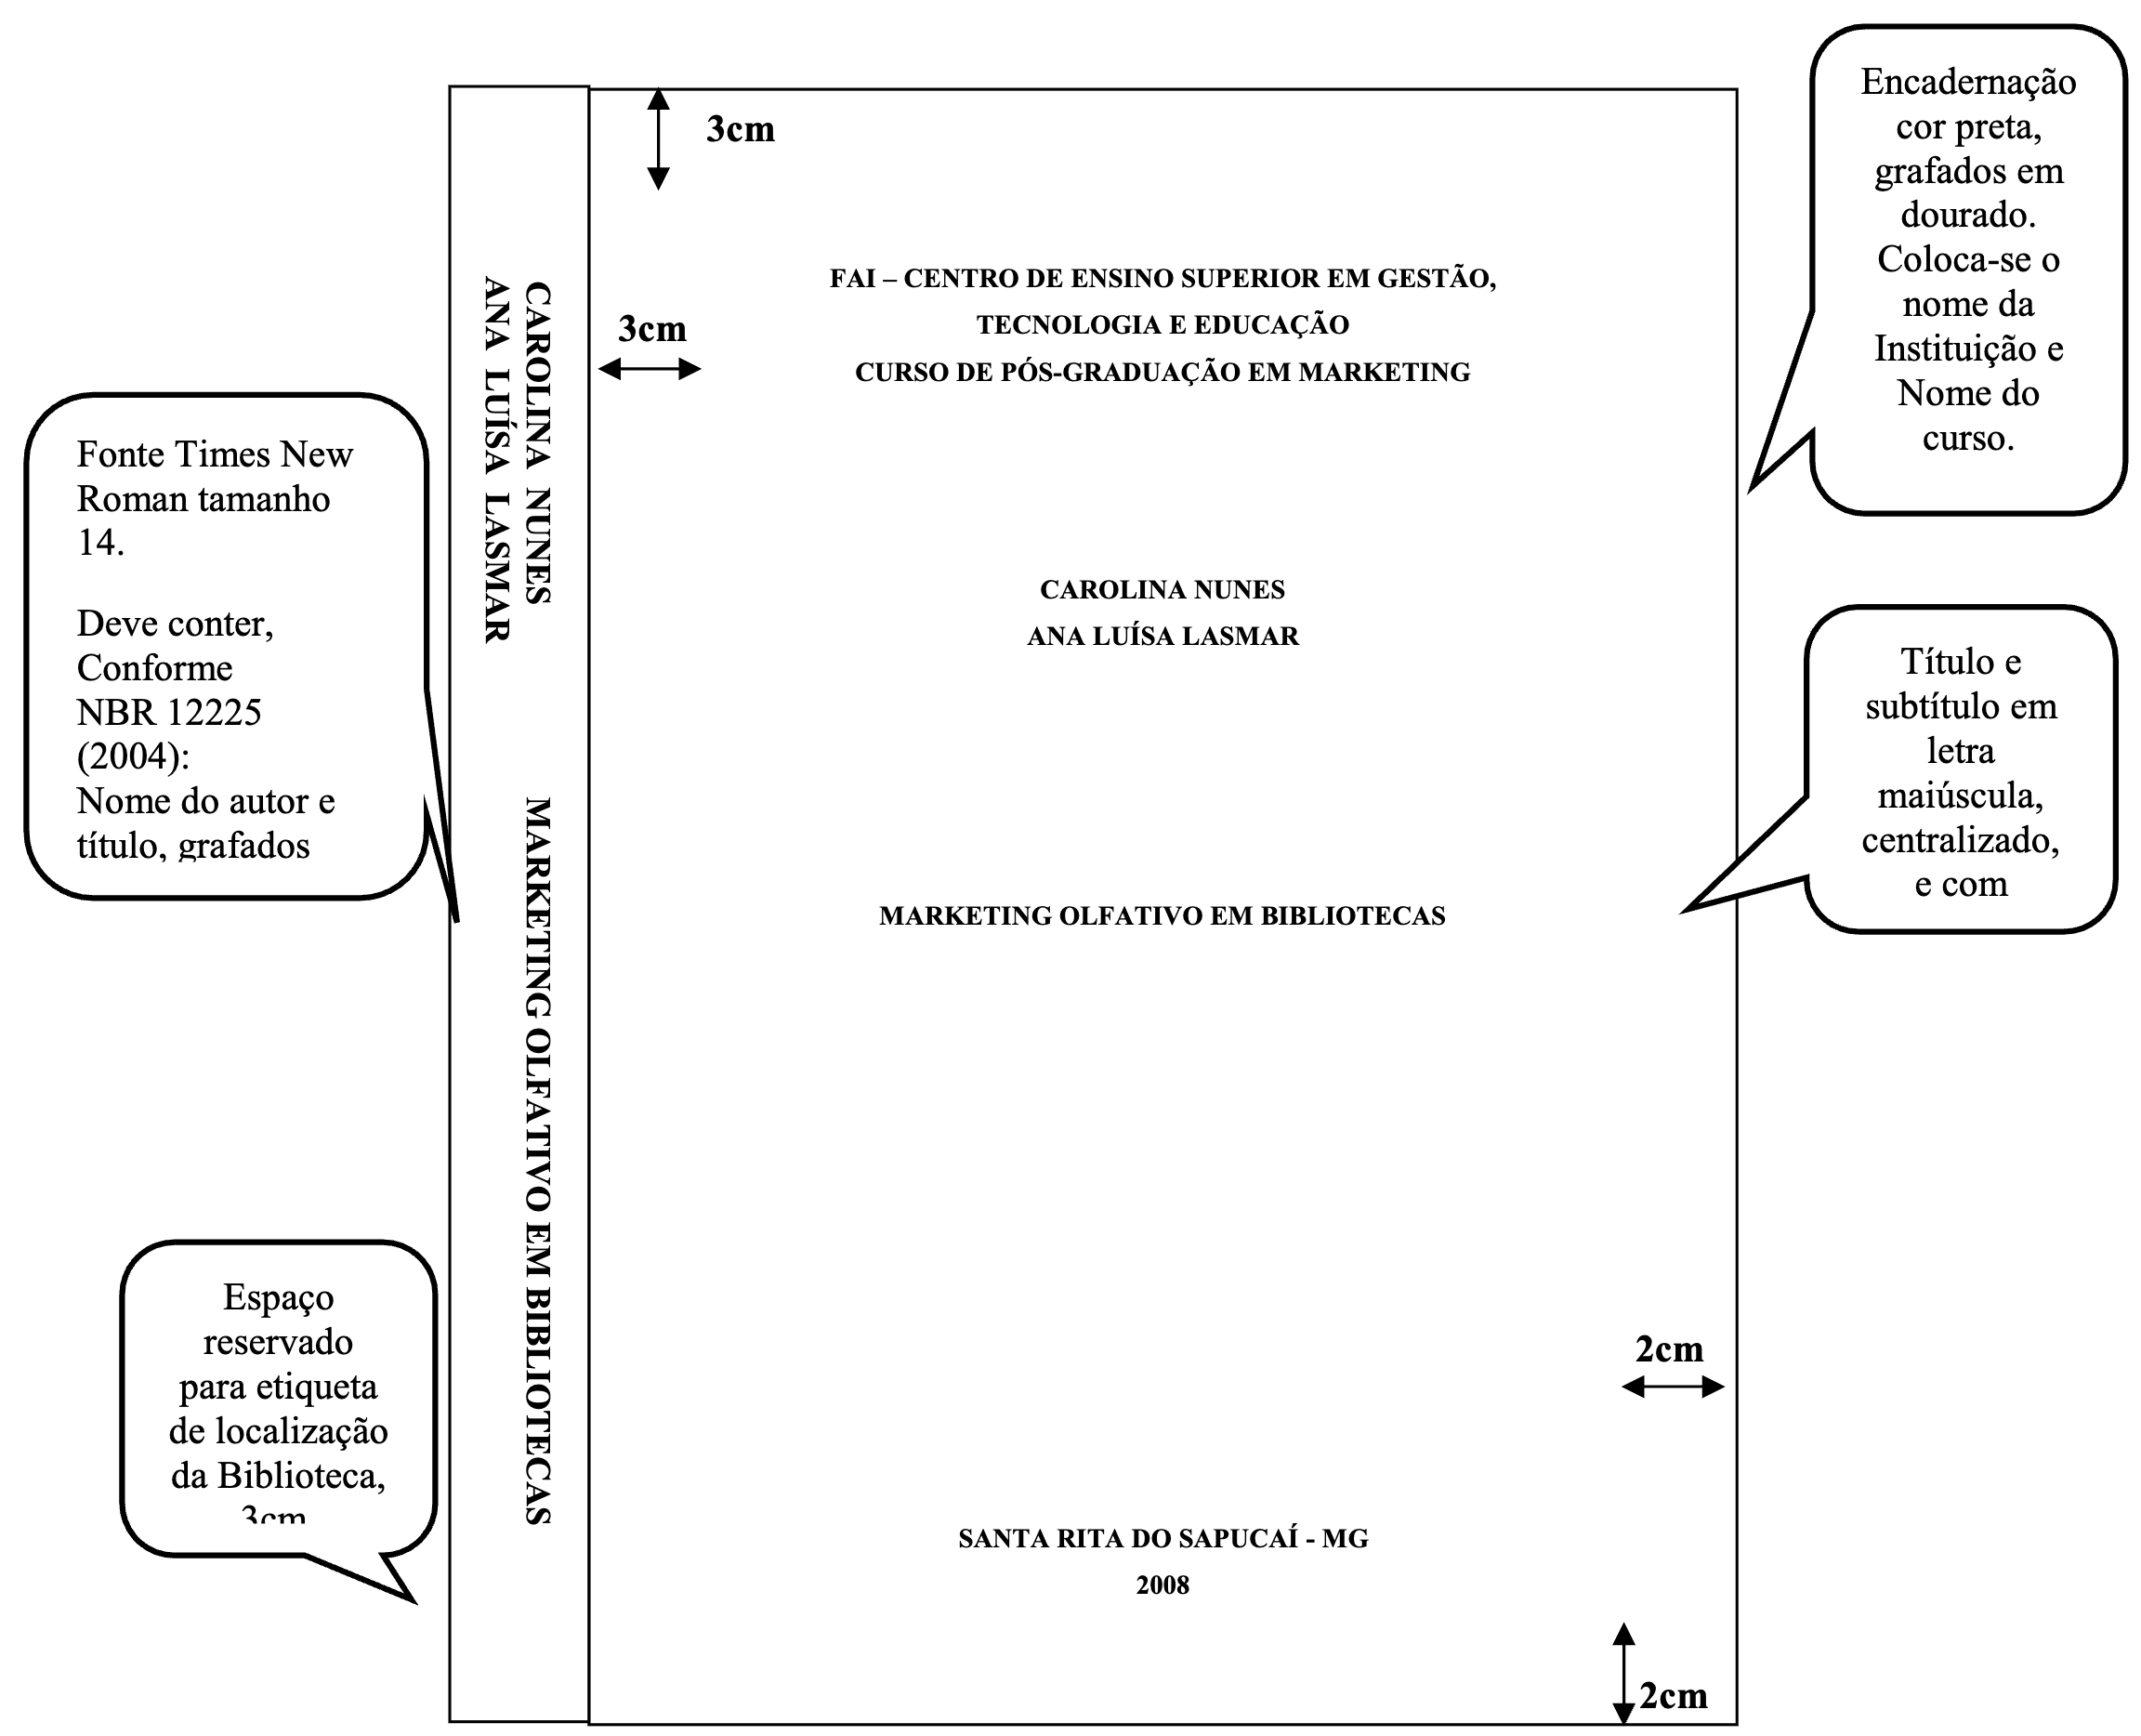
\includegraphics[width=1\textwidth]{ilustracoes/figuras/Modelo de Capa e Lombada.png}
  \legenda{Modelo de Capa e Lombada}
  \fonte{Elaboração própria}
  \label{figura:ModeloDeCapaELombada}
\end{figura}

\secaoterciaria{Capa dura e encadernação (Condicional)}
"Capa de proteção externa do trabalho sobre o qual se imprimem as informações indispensáveis à sua identificação", conforme NBR 14724 (ABNT, 2011, p. 2). A capa dura deve conter os mesmos elementos e disposição dos dados da capa ou falsa folha de rosto. Em caso de Monografia e documentação de Trabalho de Conclusão de Curso (TCC), a cópia definitiva deve ser feita com capa dura, na cor preta, com inscrições na cor dourada, para ser arquivada na Biblioteca da FAI. Os demais trabalhos devem ser encadernados com capa de plástico transparente incolor, contra capa preta e espiral também preta, ou conforme solicitação do docente.

O modelo de Capa e Lombada apresentado pela Figura 2 usa fonte de tamanho menor e serve apenas para visualização do conteúdo da folha. Os demais modelos encontram-se nos Apêndices B até Apêndice M.

A capa deve conter:
\begin{alinea}
  \item nome da Instituição;
  \item nome do curso;
  \item nome do autor;
  \item título do trabalho;
  \item subtítulo (se houver); deve ser evidenciada a sua subordinação ao título principal, precedido de dois pontos ( : );
  \item local (cidade) da instituição onde deve ser apresentado;
  \item ano de depósito (da entrega), se TCC, monografia, artigo, dissertação ou tese. Caso seja trabalho técnico-científico para avaliação bimestral ou parte deste, colocar mês/ano da entrega.
\end{alinea}

\secaosecundaria{Elementos Pré-Textuais}
Os elementos pré-textuais são apresentados pela Figura \ref{figura:ElementosPreTextuais} e nas seções seguintes.

\begin{figura}[h!]
  \centering
  \addfigura
  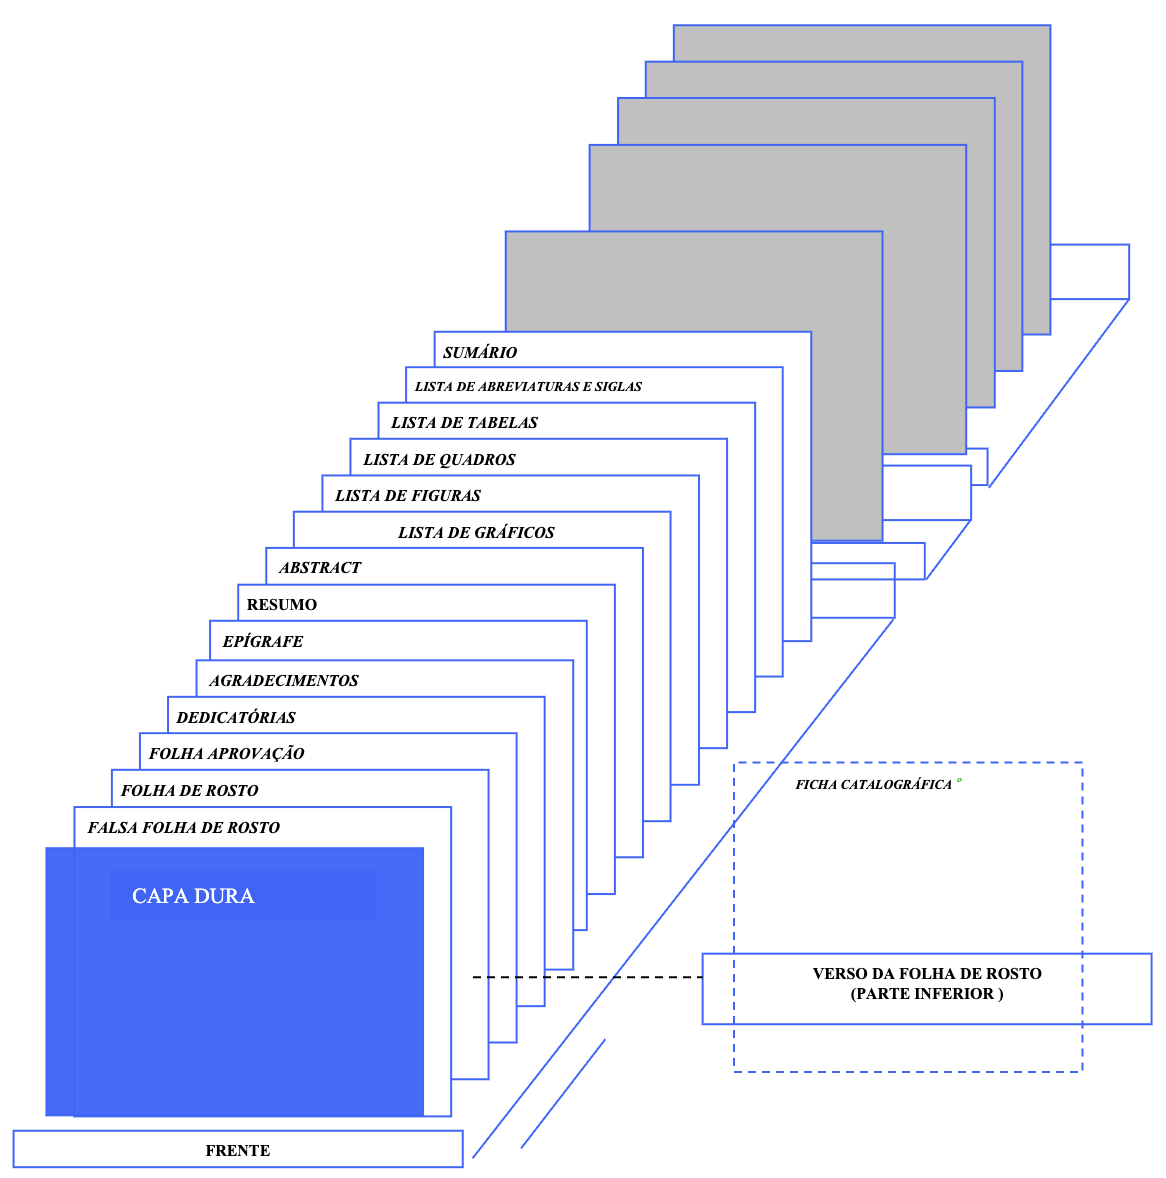
\includegraphics[width=1\textwidth]{ilustracoes/figuras/Elementos Pre Textuais.png}
  \legenda{Elementos Pré-Textuais}
  \fonte{Elaboração própria}
  \label{figura:ElementosPreTextuais}
\end{figura}

\secaoterciaria{Capa ou falsa folha de rosto (Obrigatórios)}
A capa, ou falsa folha de rosto, deve conter dados que permitam a correta identificação do trabalho: nome da Instituição, do curso, do(s) autor(es), título do trabalho e subtítulos, local e data, conforme mostra o Apêndice B.

% FIM: DESENVOLVIMENTO ================================================================
\end{Desenvolvimento}

\begin{Conclusao} % ------------------------------------------------------------------
\secaoprimaria{Conclusão}
% ============================================================================
% DESENVOLVIMENTO- EDITE O TEXTO ABAIXO. É O CONTEÚDO PRINCIPAL DO TRABALHO
% ============================================================================
...

% FIM: CONCLUSÃO==============================================================
\end{Conclusao}
\end{ElementosTextuais}

% ====== ELEMENTOS PÓS-TEXTUAIS ===================================================
\begin{ElementosPosTextuais}
\begin{Referencias} % ----------------------------------------------------------------
\end{Referencias}


% ============================================================================
% (NÃO EDITAR) GLOSSÁRIO - EDITE O ARQUIVO glossario.tex SE NECESSÁRIO
% ============================================================================
\ifdefstring{\tipodedocumento}{Monografia}{% ======================================================================================
% Glossário - Definição do Glossário
% Comente (com % antes do texto) o conteúdo abaixo para não exibir a epigrafe
%
% Relação de palavras ou expressões técnicas de uso restrito ou de sentido obscuro, 
%    utilizadas no texto, acompanhadas das respectivas definições
%
% Glossário PODE ser usado em Monografias
% ======================================================================================

\begin{Glossario}
    % Adicione termos e definições no formato \glossario{TERMO}{DEFINIÇÃO}
    \glossario{Abreviatura}{representação de uma palavra por meio de alguma(s) de suas sílabas ou letras.}
    \glossario{Agradecimento}{são expressões de gratidão às pessoas que contribuíram efetivamente para o desenvolvimento do trabalho.}
    \glossario{Análise e Discussão dos Resultados}{parte do desenvolvimento que tem a função de analisar e interpretar os dados obtidos nos procedimentos metodológicos levando em conta o referencial teórico. Pode haver uma comparação entre a prática e a teoria, apresentando no que ambas se completam, se corroboram ou se contradizem. Os gráficos estatísticos e os relatos de testes e validações são analisados e comentados, analisando se as informações e provas obtidas confirmam ou rejeitam as hipóteses.}
    \glossario{Anexo}{texto ou documento não elaborado pelo autor, que serve de fundamentação, comprovação e complementa o trabalho. São anexos também os trabalhos do próprio autor, porém não realizados especificamente para o trabalho atual.}
    \glossario{Apêndice}{texto ou documento elaborado pelo autor para o trabalho atual, a fim de complementar sua argumentação, sem prejuízo da unidade nuclear do texto.}
    \glossario{Apuddo}{do latim, significa “citado por”, “conforme”, “segundo”.}
    \glossario{Artigo}{e revisão: Parte de uma publicação que resume, analisa e discute informações já publicadas.}
    \glossario{Artigo}{riginal: Parte de uma publicação que apresenta temas ou abordagens originais.}
    \glossario{Autor-entidade}{quando o autor não é uma pessoa física, mas, sim, instituição(ões), organização(ões), empresa(s), comitê(s), comissão(ões), evento(s), entre outros, responsável(eis) por publicações em que não se distingue autoria pessoal.}
    \glossario{Bibliografia}{conjunto de livros sobre um assunto.}
    \glossario{Capa}{proteção externa do trabalho e sobre a qual se imprimem as informações para a sua identificação.}
\end{Glossario}}{}

\begin{Apendice} % -----------------------------------------------------------------
\end{Apendice}

\begin{Anexo} % --------------------------------------------------------------------
\end{Anexo}

\begin{Indice} % --------------------------------------------------------------------
\end{Indice}

% ===================================================================================
\end{ElementosPosTextuais}

\end{document}